\documentclass{beamer}

\usepackage{comment}
\usepackage{color}
\usepackage{listings}
\usepackage{verbatim}
\usepackage{multicol}
\usepackage{booktabs}
\usepackage{textpos}
\usepackage{graphicx}
\usepackage{graphics}
\definecolor{green}{RGB}{0,128,0}

\newcommand{\bc}{\begin{center}}
\newcommand{\ec}{\end{center}}
\newcommand{\eq}{\ =\ }
\newcommand{\degc}{$^\circ$C}

\newcommand\gehcomment[1]{{{\color{orange} #1}}}
\newcommand\add[1]{{{\color{blue} #1}}}
\newcommand\remove[1]{\sout{{\color{red} #1}}}
\newcommand\codecomment[1]{{{\color{green} #1}}}
\newcommand\redcomment[1]{{{\color{red} #1}}}
\newcommand\bluecomment[1]{{{\color{blue} #1}}}
\newcommand\greencomment[1]{{{\color{green} #1}}}
\newcommand\magentacomment[1]{{{\color{magenta} #1}}}

\begin{comment}
\tiny
\scriptsize
\footnotesize
\small
\normalsize
\large
\Large
\LARGE
\huge
\Huge
\end{comment}

\begin{document}
\title{1D Hot Steam Injection\ldots}
\author{Michael Nole}
\date{\today}

%\frame{\titlepage}

%-----------------------------------------------------------------------------
\section{Description of 1D Hot Steam Injection Scenario}

\subsection{1D Hot Steam Injection Conceptual Model}

\frame{\frametitle{Description of 1D Hot Steam Injection Flow Scenario}

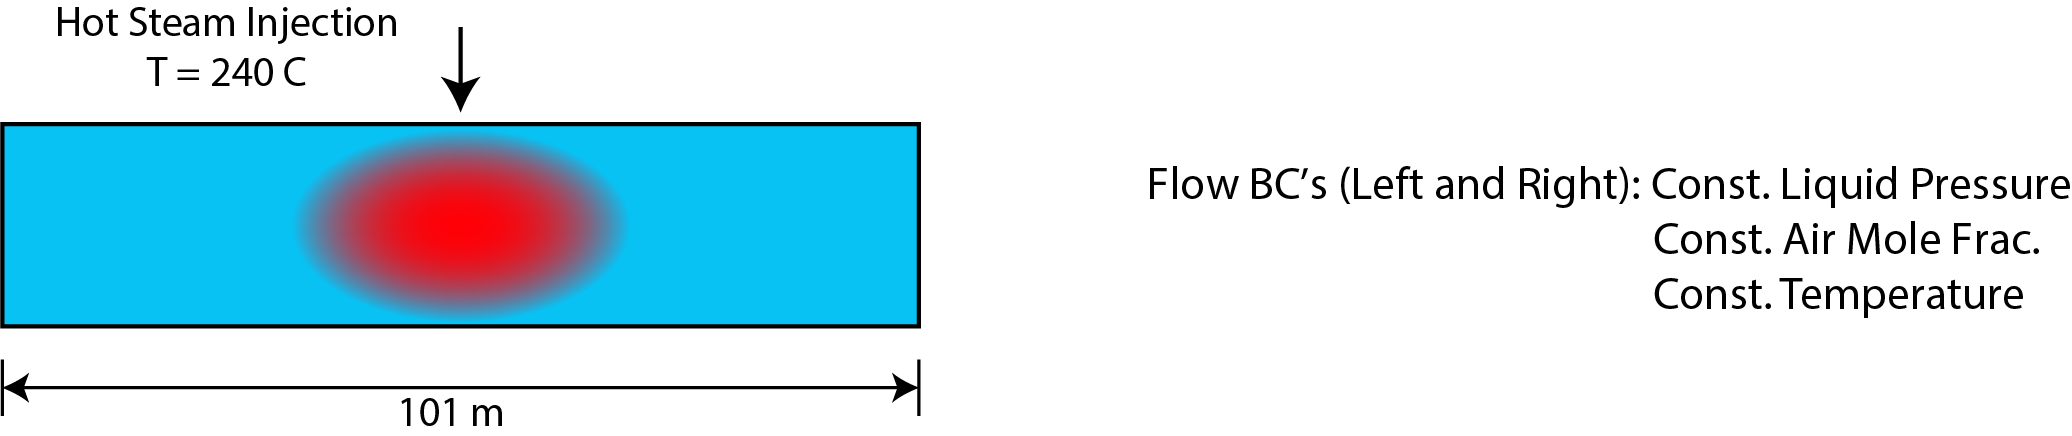
\includegraphics[height=0.8in]{./hot_steam_injection.png}

The ``1D Hot Steam Injection Scenario'' simulates injection of hot steam into the center of a water-saturated domain using \redcomment{GENERAL MODE}. This scenario demonstrates how to make use of different GENERAL mode options to optimize simulation performance.
\begin{itemize}
  \small
  \item Problem domain: $101 \times 1 \times 1$ m (x $\times$ y $\times$ z)
  \item Grid resolution $1 \times 1 \times 1$ m
  \item Initial liquid pressure of 1 MPa, temperature of 176C
  \item Inject water at a constant Mass Rate of 5 mg/sec, air at 0.05 mg/s  
  \item Material properties
  \begin{itemize}
    \footnotesize
    \item $k \eq 10^{-14}$ [m$^2$]
    \item $\varphi \eq 0.25$
    \item Saturation function: Brooks-Corey
  \end{itemize}
  \item Total simulation time: 5 y
\end{itemize}
}

%-----------------------------------------------------------------------------
\section{Description of Input Deck}

%-----------------------------------------------------------------------------
\subsection{SIMULATION}

\begin{frame}[fragile]\frametitle{SIMULATION}

\begin{itemize}
\item Specify General flow mode
\item Start by using the default options
\end{itemize}


\begin{semiverbatim}

SIMULATION
  SIMULATION_TYPE SUBSURFACE
  PROCESS_MODELS
    SUBSURFACE_FLOW flow
      MODE GENERAL
    /
  /
END

SUBSURFACE
 ...
END_SUBSURFACE
\end{semiverbatim}

\end{frame}

%-----------------------------------------------------------------------------
\subsection{GRID}
\begin{frame}[fragile,containsverbatim]\frametitle{GRID}

\begin{itemize}
  \item Problem domain: $101 \times 1 \times 1$ m (x $\times$ y $\times$ z)
  \item Grid resolution $1 \times 1 \times 1$ m
\end{itemize}

\begin{semiverbatim}
GRID
  TYPE STRUCTURED        \bluecomment{! structured grid}
  NXYZ 101 1 1           \bluecomment{! NX, NY, NZ}
  DXYZ            
    101@1.d0   \bluecomment{! Nx @ dX}
    1@1.d0  \bluecomment{! Ny @ dY}
    1@1.d0  \bluecomment{! Nz @ dZ}
  /  
END  \bluecomment{! <-- closes out GRID card}
\end{semiverbatim}

\end{frame}

%-----------------------------------------------------------------------------
\subsection{Fluid Properties}

\begin{frame}[fragile,containsverbatim,allowframebreaks]\frametitle{Fluid Properties}

\begin{itemize}
  \item Define properties of water and gas
  \begin{itemize}
    \item Diffusion coefficients
    \item Equations of state
  \end{itemize}
\end{itemize}

\begin{semiverbatim}
FLUID_PROPERTY
  PHASE LIQUID
  DIFFUSION_COEFFICIENT 2.d-9
END

FLUID_PROPERTY
  PHASE GAS
  DIFFUSION_COEFFICIENT 2.d-5
END

\newpage

EOS WATER
  DENSITY IF97
  ENTHALPY IF97
  STEAM_DENSITY IF97
  STEAM_ENTHALPY IF97
END

EOS GAS
  DENSITY DEFAULT
  VISCOSITY DEFAULT
  HENRYS_CONSTANT DEFAULT
END

\end{semiverbatim}

\end{frame}

%-----------------------------------------------------------------------------
\subsection{MATERIAL\_PROPERTY}

\begin{frame}[fragile,containsverbatim]\frametitle{MATERIAL\_PROPERTY}

\begin{semiverbatim}
MATERIAL_PROPERTY soil1  \bluecomment{! define a material:} \greencomment{soil1}
  ID 1             \bluecomment{! material ID assigned to grid cells}
  CHARACTERISTIC\_CURVES cc1
  POROSITY 0.25d0
  TORTUOSITY 1.d0
  ROCK_DENSITY 2700.d0
  THERMAL_CONDUCTIVITY_DRY 1.1d0 W/m-C
  THERMAL_CONDUCTIVITY_WET 1.1d0 W/m-C
  HEAT_CAPACITY 0.01 J/kg-C
  PERMEABILITY     
    PERM_ISO 1.d-14  \bluecomment{! isotropic permeability}
  /
END
\end{semiverbatim}

\end{frame}

%-----------------------------------------------------------------------------
\subsection{CHARACTERISTIC\_CURVES}

\begin{frame}[fragile,containsverbatim, allowframebreaks]\frametitle{CHARACTERISTIC\_CURVES}

\begin{itemize}
\item Set Brooks-Corey parameters
\end{itemize}

\begin{semiverbatim}
CHARACTERISTIC_CURVES default
  SATURATION_FUNCTION BROOKS_COREY
    ALPHA 4.d-4
    LAMBDA 2
    LIQUID_RESIDUAL_SATURATION 0.1d0
    CALCULATE_INTERFACIAL_TENSION 
     \bluecomment{        ! Interfacial tension as f(T)}
  /
\end{semiverbatim}

\newpage
\begin{itemize}
\item Burdine relative permeability
\end{itemize}

\begin{semiverbatim}
  PERMEABILITY_FUNCTION BURDINE_BC_LIQ
    PHASE LIQUID
    LAMBDA 2
    LIQUID_RESIDUAL_SATURATION 0.1d0
  /

  PERMEABILITY_FUNCTION BURDINE_BC_GAS
    PHASE GAS
    LAMBDA 2
    LIQUID_RESIDUAL_SATURATION 0.1d0
    GAS_RESIDUAL_SATURATION 0.1d0
  /
END
\end{semiverbatim}

\end{frame}

%-----------------------------------------------------------------------------
\subsection{REGION}

\begin{frame}[fragile,containsverbatim,allowframebreaks]\frametitle{REGION}

\begin{itemize}
  \item Delineate regions in the 1D domain for:
  \begin{itemize}
    \item top boundary face
    \item bottom boundary face
    \item entire domain (all)
  \end{itemize}
\end{itemize}

\begin{semiverbatim}
REGION all            \bluecomment{! define a region and name it: \greencomment{all}}
  COORDINATES        
    0.d0 0.d0 0.d0    \bluecomment{! lower coordinate: xmin ymin zmin}
    101.d0 1.d0 1.d0   \bluecomment{! upper coordinate: xmax ymax zmax}
  /   \bluecomment{! <-- closes out COORDINATES card}
END   \bluecomment{! <-- closes out REGION card}

\newpage
REGION left            \bluecomment{! define region:} \greencomment{left}
  FACE WEST            \bluecomment{! define the face of the grid cell}
  COORDINATES         
    0.d0 0.d0 0.d0
    0.d0 1.d0 1.d0
  /
END

REGION right         \bluecomment{! define region:} \greencomment{right}
  FACE EAST         
  COORDINATES         
    101.d0 0.d0 0.d0    
    101.d0 1.d0 1.d0
  /
END

REGION injector   \bluecomment{! define region containing injection}
  COORDINATE 51.d0 0.5d0 0.5d0
/

\end{semiverbatim}

\end{frame}

%-----------------------------------------------------------------------------
\subsection{FLOW\_CONDITION}

\begin{frame}[fragile,allowframebreaks]\frametitle{FLOW\_CONDITION}

\begin{itemize}
\item Initially in \redcomment{LIQUID STATE}
\item Specify an initial pressure, aqueous air mole fraction, temperature
\end{itemize}

\begin{semiverbatim}
FLOW_CONDITION initial 
  TYPE
    LIQUID_PRESSURE DIRICHLET \bluecomment{! Conditions must be}
    MOLE_FRACTION DIRICHLET   \bluecomment{! consistent with}
    TEMPERATURE DIRICHLET     \bluecomment{! phase state}
  /
  LIQUID_PRESSURE 1.d6
  MOLE_FRACTION 0.d0
  TEMPERATURE 176.d0
END                      

\newpage

FLOW_CONDITION steam_injection 
  TYPE
    RATE MASS_RATE         \bluecomment{! Type is \redcomment{mass_rate}}
    TEMPERATURE DIRICHLET  \bluecomment{! with a constant injection}
  /                        \bluecomment{! temperature}

  TEMPERATURE 200.d0       \bluecomment{! Steam temperature is 200 C}     
  RATE 5.d-3 5.d-5 0.d0 g/s g/s MW \bluecomment{Injecting mostly water,}
END                                \bluecomment{some air}
\end{semiverbatim}

\end{frame}

%-----------------------------------------------------------------------------
\subsection{INITIAL\_CONDITION}

\begin{frame}[fragile]\frametitle{INITIAL\_CONDITION}

\begin{itemize}
\item Couple the \greencomment{initial} flow condition with region \greencomment{all} for the initial condition
\end{itemize}

\begin{semiverbatim}

INITIAL_CONDITION all 
  FLOW_CONDITION initial
  REGION all
END

\end{semiverbatim}

\end{frame}

%-----------------------------------------------------------------------------
\subsection{BOUNDARY\_CONDITION}

\begin{frame}[fragile]\frametitle{BOUNDARY\_CONDITION}

\begin{itemize}
\item Couple the \greencomment{left} and \greencomment{right} flow conditions with their corresponding regions.
\end{itemize}

\begin{semiverbatim}

BOUNDARY_CONDITION left
  FLOW_CONDITION initial
  REGION left
END

BOUNDARY_CONDITION right
  FLOW_CONDITION initial
  REGION right
END

\end{semiverbatim}

\end{frame}

%-----------------------------------------------------------------------------
\subsection{SOURCE\_SINK}

\begin{frame}[fragile]\frametitle{SOURCE\_SINK}

\begin{itemize}
	\item Couple the \greencomment{steam\_injection} flow condition with the \greencomment{injector} region.
\end{itemize}

\begin{semiverbatim}
SOURCE_SINK injector
  FLOW_CONDITION steam_injection
  REGION injector
END
\end{semiverbatim}

\end{frame}

%-----------------------------------------------------------------------------

\subsection{STRATA}

\begin{frame}[fragile]\frametitle{STRATA}

\begin{itemize}
\item Couple \greencomment{soil1} rock/soil type with region \greencomment{all} to define a stratigraphic unit
\end{itemize}

\begin{semiverbatim}

STRATA
  REGION all
  MATERIAL soil1
END


\end{semiverbatim}

\end{frame}

%-----------------------------------------------------------------------------
\subsection{OUTPUT}

\begin{frame}[fragile]\frametitle{OUTPUT}

\begin{itemize}
\item Set output times to 0.05 0.1 1.0 5.0 years
\end{itemize}


\begin{semiverbatim}

OUTPUT
  SNAPSHOT_FILE
  \magentacomment{TIMES y  .05d0 0.1d0 1.d0 5.d0}   
  FORMAT TECPLOT POINT            
END

\end{semiverbatim}

\end{frame}

%-----------------------------------------------------------------------------
\subsection{TIME}

\begin{frame}[fragile]\frametitle{TIME}

\begin{itemize}
\item Change final simulation time to 5 years
\end{itemize}

\begin{semiverbatim}

TIME
  FINAL_TIME \magentacomment{5.d0} y
  INITIAL_TIMESTEP_SIZE 1.d0 h
  MAXIMUM_TIMESTEP_SIZE 5.d-1 y
END

\end{semiverbatim}

\end{frame}

%-----------------------------------------------------------------------------
\subsection{Running hot_steam_injection.in}

\begin{frame}[fragile]\frametitle{Running PFLOTRAN}

\begin{semiverbatim}

> cd $PFLOTRAN_DIR
> cd shortcourse/exercises/1D_hot_steam_injection
> pflotran -input_prefix hot_steam_injection
> CTRL-C \bluecomment{! to stop simulation}
\end{semiverbatim}

\end{frame}

%-----------------------------------------------------------------------------
\subsection{Ouput Messages 1}

\begin{frame}[fragile]\frametitle{Screen Output}

\begin{semiverbatim}
\tiny
== GENERAL MULTIPHASE FLOW =====================================================
  0 2r: 4.45E-06 2x: 0.00E+00 2u: 0.00E+00 ir: 2.95E-06 iu: 0.00E+00 rsn:   0
 (0): State Transition: Liquid -> 2 Phase at Cell       39
 (0): State Transition: Liquid -> 2 Phase at Cell       63
  1 2r: 1.63E-04 2x: 1.01E+07 2u: 5.71E+02 ir: 9.12E-05 iu: 9.63E+01 rsn:   0
 (0): State Transition: 2 Phase -> Liquid at Cell       39
 (0): State Transition: 2 Phase -> Liquid at Cell       63
  2 2r: 2.06E-04 2x: 1.01E+07 2u: 2.04E+03 ir: 1.18E-04 iu: 1.44E+03 rsn:   0
 (0): State Transition: Liquid -> 2 Phase at Cell       39
 (0): State Transition: Liquid -> 2 Phase at Cell       63
  3 2r: 1.58E-04 2x: 1.01E+07 2u: 2.03E+03 ir: 8.77E-05 iu: 1.29E+03 rsn:   0
 (0): State Transition: 2 Phase -> Liquid at Cell       39
 (0): State Transition: 2 Phase -> Liquid at Cell       63
  4 2r: 2.06E-04 2x: 1.01E+07 2u: 2.03E+03 ir: 1.18E-04 iu: 1.30E+03 rsn:   0
 (0): State Transition: Liquid -> 2 Phase at Cell       39
 (0): State Transition: Liquid -> 2 Phase at Cell       63
  5 2r: 1.58E-04 2x: 1.01E+07 2u: 2.03E+03 ir: 8.77E-05 iu: 1.30E+03 rsn:   0
 (0): State Transition: 2 Phase -> Liquid at Cell       39
 (0): State Transition: 2 Phase -> Liquid at Cell       63
  6 2r: 2.06E-04 2x: 1.01E+07 2u: 2.03E+03 ir: 1.18E-04 iu: 1.30E+03 rsn:   0
 (0): State Transition: Liquid -> 2 Phase at Cell       39
 (0): State Transition: Liquid -> 2 Phase at Cell       63
  7 2r: 1.58E-04 2x: 1.01E+07 2u: 2.03E+03 ir: 8.77E-05 iu: 1.30E+03 rsn:   0
 (0): State Transition: 2 Phase -> Liquid at Cell       39
 (0): State Transition: 2 Phase -> Liquid at Cell       63
  8 2r: 2.06E-04 2x: 1.01E+07 2u: 2.03E+03 ir: 1.18E-04 iu: 1.30E+03 rsn:   0
 (0): State Transition: Liquid -> 2 Phase at Cell       39
 (0): State Transition: Liquid -> 2 Phase at Cell       63
  9 2r: 1.58E-04 2x: 1.01E+07 2u: 2.03E+03 ir: 8.77E-05 iu: 1.30E+03 rsn:   0
 (0): State Transition: 2 Phase -> Liquid at Cell       39
 (0): State Transition: 2 Phase -> Liquid at Cell       63

\end{semiverbatim}


\end{frame}

%-----------------------------------------------------------------------------
\subsection{Edit the Input Deck 1}

\begin{frame}[fragile]\frametitle{Edit the Input Deck}

\begin{semiverbatim}

SIMULATION
  SIMULATION_TYPE SUBSURFACE
  PROCESS_MODELS
    SUBSURFACE_FLOW flow
      MODE GENERAL ! two-phase flow and energy
      OPTIONS
        RESTRICT_STATE_CHANGE
      /
    /
  /
END

\end{semiverbatim}

\end{frame}
%-----------------------------------------------------------------------------
\subsection{Running hot_steam_injection.in again}

\begin{frame}[fragile]\frametitle{Running PFLOTRAN}

\begin{semiverbatim}

> cd $PFLOTRAN_DIR
> cd shortcourse/exercises/1D_hot_steam_injection
> pflotran -input_prefix hot_steam_injection
> python hot_steam_injection.py
\end{semiverbatim}

\end{frame}

%-----------------------------------------------------------------------------
\subsection{Edit the Input Deck 2}

\begin{frame}[fragile]\frametitle{Edit the Input Deck (again)}

\begin{semiverbatim}
>Simulation block  remains the same
>Add a numerical methods block 
  >Newton Solver sub-block

NUMERICAL_METHODS FLOW
  NEWTON_SOLVER
    NUMERICAL_JACOBIAN
  /
END

\end{semiverbatim}

\end{frame}

%-----------------------------------------------------------------------------
\subsection{Running hot_steam_injection.in 3}

\begin{frame}[fragile]\frametitle{Running PFLOTRAN}

\begin{semiverbatim}

> cd $PFLOTRAN_DIR
> cd shortcourse/exercises/1D_hot_steam_injection
> pflotran -input_prefix hot_steam_injection
> CTRL-C
\end{semiverbatim}

\end{frame}

%-----------------------------------------------------------------------------
\subsection{Edit the Input Deck 3}

\begin{frame}[fragile]\frametitle{Edit the Input Deck (again)}

\begin{semiverbatim}
>Simulation block remains the same
>Edit numerical methods block

NUMERICAL_METHODS FLOW
  NEWTON_SOLVER
    NUMERICAL_JACOBIAN
    USE_INFINITY_NORM_CONVERGENCE
  /
END

\end{semiverbatim}

\end{frame}
%-----------------------------------------------------------------------------
\subsection{Running hot_steam_injection.in again}

\begin{frame}[fragile]\frametitle{Running PFLOTRAN}

\begin{semiverbatim}

> cd $PFLOTRAN_DIR
> cd shortcourse/exercises/1D_hot_steam_injection
> pflotran -input_prefix hot_steam_injection
> python hot_steam_injection.py
\end{semiverbatim}

\end{frame}

\end{document}
